\begin{frame}
	\myheading{Module 2.3: Perceptron}
\end{frame}

\begin{frame}
	\begin{block}{The story ahead ...}
		\onslide<1->{
			\begin{itemize}\justifying
				\item<1-> What about non-boolean (say, real) inputs ?
				\item<2-> Do we always need to hand code the threshold ?
				\item<3-> Are all inputs equal ? What if we want to assign more weight (importance) to some inputs ?
				\item<4-> What about functions which are not linearly separable ?
			\end{itemize}
		}
	\end{block}
\end{frame}

\begin{frame}
	\begin{columns}
		\column{0.4\textwidth}
		\begin{overlayarea}{\textwidth}{\textheight}
			%\begin{center}
			\begin{center}
				\onslide<2->{
					\begin{tikzpicture}
	\node (input0) at (8,-0.1)  {$x_{1}$};
	\node (input1) at (9,-0.1)  {$x_{2}$};
	\node (input2) at (10,-0.1)  {$..$};
	\node (input3) at (11,-0.1)  {$..$};
	\node (input4) at (12,-0.1)  {$x_{n}$};

	\node [hidden_neuron] (neuron1) at (10,2)  {};

	\node (output0)  at (10,3.5) {$y$};

	\draw [->] (input0) -- (neuron1);
	\draw [->] (input1) -- (neuron1);
	\draw [->] (input2) -- (neuron1);
	\draw [->] (input3) -- (neuron1);
	\draw [->] (input4) -- (neuron1);

	\draw [->] (neuron1) -- (output0);

	\node (formula)[scale=.8] at (8.1,0.6) {$w_{1}$};
	\node (formula)[scale=.8] at (9.1,0.6) {$w_{2}$};
	\node (formula)[scale=.8] at (9.8,0.6) {$..$};
	\node (formula)[scale=.8] at (10.4,0.6) {$..$};
	\node (formula)[scale=.8] at (11.1,0.6) {$w_{n}$};
\end{tikzpicture}


				}
				%\end{center}

			\end{center}
		\end{overlayarea}

		\column{0.6\textwidth}
		\begin{overlayarea}{\textwidth}{\textheight}
			\begin{itemize}\justifying
				\item<1-> Frank Rosenblatt, an American psychologist, proposed the \textbf{classical perceptron} model (1958)
				\item<3-> A more general computational model than McCulloch–Pitts neurons
				\item<4-> \textbf{Main differences:} Introduction of numerical weights for inputs and a mechanism for learning these weights
				\item<5-> Inputs are no longer limited to boolean values
				\item<6-> Refined and carefully analyzed by Minsky and Papert (1969) - their model is referred to as the \textbf{perceptron} model here
			\end{itemize}
		\end{overlayarea}
	\end{columns}
\end{frame}



\begin{frame}
	\begin{columns}
		\column{0.4\textwidth}
		\begin{overlayarea}{\textwidth}{\textheight}
			\begin{center}
				\begin{tikzpicture}
	\node (input0) at (8,-0.1)  {$x_{1}$};
	\node (input1) at (9,-0.1)  {$x_{2}$};
	\node (input2) at (10,-0.1)  {$..$};
	\node (input3) at (11,-0.1)  {$..$};
	\node (input4) at (12,-0.1)  {$x_{n}$};
	\onslide<10->{\node (input5) at (7,-0.1)  {$\color{red}{x_{0}=1}$};}

	\node [hidden_neuron] (neuron1) at (10,2)  {};


	\node (output0)  at (10,3.5) {$y$};

	\draw [->] (input0) -- (neuron1);
	\draw [->] (input1) -- (neuron1);
	\draw [->] (input2) -- (neuron1);
	\draw [->] (input3) -- (neuron1);
	\draw [->] (input4) -- (neuron1);
	\onslide<10->{\draw [->, red] (input5) -- (neuron1);}

	\draw [->] (neuron1) -- (output0);

	\node (formula)[scale=.8] at (8.4,0.6) {$w_{1}$};
	\node (formula)[scale=.8] at (9.1,0.6) {$w_{2}$};
	\node (formula)[scale=.8] at (9.8,0.6) {$..$};
	\node (formula)[scale=.8] at (10.4,0.6) {$..$};
	\node (formula)[scale=.8] at (11.1,0.6) {$w_{n}$};
	\onslide<10->{\node (formula)[scale=.8] at (7.2,0.6) {$\color{red}{w_{0} = -\theta}$};}

\end{tikzpicture}
			\end{center}
			\vspace{-0.2in}
			\onslide<7->{A more accepted convention,}
			\vspace{-0.1in}
			\begin{align*}
				\onslide<8->{y                & =1 \quad if \sum^{n}_{\color{red}{i=0}} w_i * x_i \geq 0} \\
				\onslide<11->{                & =0  \quad if \sum^{n}_{\color{red}{i=0}} w_i * x_i < 0}   \\
				\onslide<9->{where, \quad x_0 & = 1 \quad and \quad w_0 = -\theta}
			\end{align*}
		\end{overlayarea}

		\column{0.6\textwidth}
		\begin{overlayarea}{\textwidth}{\textheight}
			\begin{align*}
				\onslide<2->{y & =1 \quad if \sum^{n}_{\color{red}{i=1}} w_i * x_i \geq \theta}     \\
				\onslide<3->{  & =0  \quad if \sum^{n}_{\color{red}{i=1}} w_i * x_i < \theta}
				\onslide<4->{\intertext{Rewriting the above,}}
				\onslide<5->{y & =1 \quad if \sum^{n}_{\color{red}{i=1}} w_i * x_i - \theta \geq 0} \\
				\onslide<6->{  & =0  \quad if \sum^{n}_{\color{red}{i=1}} w_i * x_i -\theta < 0}
			\end{align*}
		\end{overlayarea}
	\end{columns}
\end{frame}

\begin{frame}
	We will now try to answer the following questions:
	\begin{itemize}\justifying
		\item Why are we trying to implement boolean functions?
		\item Why do we need weights ?
		\item Why is $w_0 = -\theta$ called the bias ?
	\end{itemize}
\end{frame}


\begin{frame}
	\begin{columns}

		\column{0.3\textwidth}
		\begin{overlayarea}{\textwidth}{\textheight}
			\begin{center}
				\begin{tikzpicture}
	\node (input5) at (7.5,-0.1)  {$x_{0}=1$};
	\node (input0) at (9,-0.1)  {$x_1$};
	%\node (input1) at (9,-0.1)  {$x_{2}$};
	\node (input2) at (10.5,-0.1)  {$x_2$};
	%\node (input3) at (11,-0.1)  {$..$};
	\node (input4) at (11.8,-0.1)  {$x_3$};

	\node [hidden_neuron] (neuron1) at (10,2)  {};


	\node (output0)  at (10,3.5) {$y$};

	\draw [->] (input0) -- (neuron1);
	%\draw [->] (input1) -- (neuron1);
	\draw [->] (input2) -- (neuron1);
	%\draw [->] (input3) -- (neuron1);
	\draw [->] (input4) -- (neuron1);
	\draw [->] (input5) -- (neuron1);

	\draw [->] (neuron1) -- (output0);

	\node (formula)[scale=.8] at (7.6,0.6) {$w_{0} = -\theta$};
	\node (formula)[scale=.8] at (9.0,0.6) {$w_{1}$};
	%\node (formula)[scale=.8] at (9.1,0.6) {$w_{2}$};
	\node (formula)[scale=.8] at (10.1,0.6) {$w_{2}$};
	%\node (formula)[scale=.8] at (10.4,0.6) {$..$};
	\node (formula)[scale=.8] at (10.9,0.6) {$w_{3}$};
\end{tikzpicture}
			\end{center}
			\onslide<3->{
				\begin{align*}
					x_1 = isActorDamon    \\
					x_2 = isGenreThriller \\
					x_3 = isDirectorNolan \\
				\end{align*}
			}
		\end{overlayarea}
		\column{0.7\textwidth}
		\begin{overlayarea}{\textwidth}{\textheight}
			\only<1-4>{
				\begin{itemize}\justifying
					\item<1-> Consider the task of predicting whether we would like a movie or not
					\item<2-> Suppose, we base our decision on 3 inputs (binary, for simplicity)
					\item<3-> Based on our past viewing experience (\textbf{data}), we may give a high weight to \textit{isDirectorNolan} as compared to the other inputs
					\item<4-> Specifically, even if the actor is not \textit{Matt Damon} and the genre is not \textit{thriller} we would still want to cross the threshold $\theta$ by assigning a high weight to \textit{isDirectorNolan}
				\end{itemize}
			}
			\only<5->{
				\begin{itemize}\justifying
					\item<5-> $w_0$ is called the bias as it represents the prior (prejudice)
					\item<6-> A movie buff may have a very low threshold and may watch any movie irrespective of the genre, actor, director [$\theta = 0$]
					\item<7-> On the other hand, a selective viewer may only watch thrillers starring Matt Damon and directed by Nolan [$\theta = 3$]
					\item<8-> The weights ($w_1, w_2, ..., w_n$) and the bias ($w_0$) will depend on the data (viewer history in this case)
				\end{itemize}
			}
		\end{overlayarea}
	\end{columns}
\end{frame}

\begin{frame}
	What kind of functions can be implemented using the perceptron? Any difference from McCulloch Pitts neurons?
\end{frame}


\begin{frame}
	\begin{columns}
		\column{0.4\textwidth}
		\begin{overlayarea}{\textwidth}{\textheight}
			\textbf{McCulloch Pitts Neuron}\\
			(assuming no inhibitory inputs)
			\begin{align*}
				y & =1 \quad if \sum^{n}_{i=0} x_i \geq \theta \\
				  & =0  \quad if \sum^{n}_{i=0} x_i < \theta   \\
			\end{align*}
			\textbf{Perceptron}
			\begin{align*}
				y & =1 \quad if \sum^{n}_{i=0} \color{red}{w_i} \color{black}{} * x_i \geq \theta \\
				  & =0  \quad if \sum^{n}_{i=0} \color{red}{w_i} \color{black}{} * x_i < \theta   \\
			\end{align*}
		\end{overlayarea}
		\column{0.6\textwidth}
		\begin{overlayarea}{\textwidth}{\textheight}
			\begin{itemize}\justifying
				\item<2-> From the equations it should be clear that even a perceptron separates the input space into two halves
				\item<3-> All inputs which produce a 1 lie on one side and all inputs which produce a 0 lie on the other side
				\item<4-> In other words, a single perceptron can only be used to implement linearly separable functions
				\item<5-> Then what is the difference? \onslide<6->{The weights (including threshold) can be learned and the inputs can be real valued}
				\item<7-> We will first revisit some boolean functions and then see the perceptron learning algorithm (for learning weights)
			\end{itemize}
		\end{overlayarea}
	\end{columns}
\end{frame}

\begin{frame}
	\begin{columns}
		\column{0.6\textwidth}
		\begin{overlayarea}{\textwidth}{\textheight}
			\begin{center}
				\begin{table}
					\begin{tabular}{cccc}
						\hline
						$x_1$ & $x_2$ & OR  \\\hline
						$0$               & $0$               & \onslide<2->{0} & \onslide<3->{$w_0 + \sum_{i=1}^{2} w_i x_i} \onslide<4->{< 0}$ \\
						\onslide<5->{$1$} & \onslide<5->{$0$} & \onslide<5->{1} & \onslide<6->{$w_0 + \sum_{i=1}^{2} w_i x_i \geq 0$}            \\
						\onslide<7->{$0$} & \onslide<7->{$1$} & \onslide<7->{1} & \onslide<8->{$w_0 + \sum_{i=1}^{2} w_i x_i \geq 0$}            \\
						\onslide<9->{$1$} & \onslide<9->{$1$} & \onslide<9->{1} & \onslide<9->{$w_0 + \sum_{i=1}^{2} w_i x_i \geq 0$}            \\
						\hline
					\end{tabular}
				\end{table}
				\begin{align*}
					\onslide<10->{w_0 + w_1\cdot0 + w_2\cdot0 < 0    & \implies w_0 < 0}          \\
					\onslide<11->{w_0 + w_1\cdot0 + w_2\cdot1 \geq 0 & \implies w_2 > -w_0}       \\
					\onslide<12->{w_0 + w_1\cdot1 + w_2\cdot0 \geq 0 & \implies w_1 > -w_0}       \\
					\onslide<13->{w_0 + w_1\cdot1 + w_2\cdot1 \geq 0 & \implies w_1 + w_2 > -w_0}
				\end{align*}

			\end{center}

			\begin{itemize}\justifying
				\item<14-> One possible solution to this set of inequalities is $w_0=-1, w_1=1.1,, w_2=1.1$ (and various other solutions are possible)
				      %\item Note that we can come up with a similar set of inequalities and found the value of $\theta$ for McCulloch Pitts neuron also
			\end{itemize}

		\end{overlayarea}
		\column{0.4\textwidth}
		\begin{overlayarea}{\textwidth}{\textheight}
			\onslide<15->{
				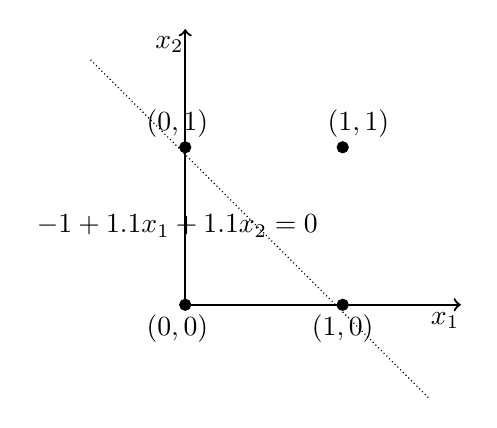
\begin{tikzpicture}
	\draw[thick,->] (0,0) -- (3.5,0);
	\draw[thick,->] (0,0) -- (0,3.5);
	\onslide<16->{\draw[densely dotted] (-1.2021,3.1111) -- (3.1111,-1.2021);}

	\node at (3.3, -0.2) {$x_1$};
	\node at (-0.2, 3.3) {$x_2$};

	\node at (-0.1, -0.3) {$(0,0)$};
	\node at (-0.1, 2.3) {$(0,1)$};
	\node at (2.0, -0.3) {$(1,0)$};
	\node at (2.2, 2.3) {$(1,1)$};
	\onslide<16->{\node at (-0.1, 1.0) {$-1 + 1.1x_1 + 1.1x_2 = 0$};}

	\filldraw (0,0) circle (2pt);
	\filldraw (0,2) circle (2pt);
	\filldraw (2,0) circle (2pt);
	\filldraw (2,2) circle (2pt);
\end{tikzpicture}
			}
			\begin{itemize}\justifying
				\item<17-> Note that we can come up with a similar set of inequalities and find the value of $\theta$ for a McCulloch Pitts neuron also \onslide<18->{(Try it!)}
			\end{itemize}
		\end{overlayarea}
	\end{columns}
\end{frame}
